\section{Приложение} \label{Приложение}

\subsection{Экспериментальная установка}
Схема экспериментальной установки приведена на рис. 1
\begin{figure}[ht]
    \center{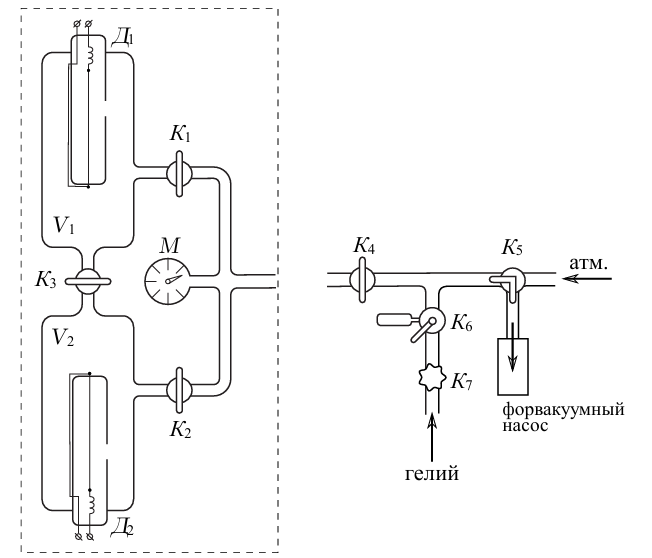
\includegraphics[scale=0.7]{img/exp_ustanovka.png}}
    \begin{center}       
        Рис. 1. Экспериментальная установка
    \end{center}
\end{figure}
Установка состоит из двух сосудов, объемами $V_1=V_2=(775 \pm 10)\text{{см}}^3$, размещенных вертикально. Краны $K_1$ и $K_2$ служат для управления откачкой о подачей воздуха/гелия в сосуды.Диффузия осуществляется через тонкую короткую трубку, соединяющую сосуды, оснащенную краном $K_3$. Выравнивание давлений в сосудах без изменения состава газов в них может быть осуществлено через обводные трубки, посредством кратковременного открытия кранов $K_1$ и $K_2$ (при закрытом $K_3$).

Гелий содержится в баллоне под давлением, превышающим атмосферное. Для предотвращения избыточного расхода гелия и его неконтролируемого проникания в установку предусмотрен кран $K_7$, отделяющий ее от баллона с гелием.Для подачи малых порций гелия предусмотрен двухходовый кран с дозатором (рис. 2).
\begin{center}
    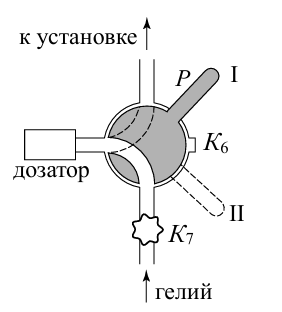
\includegraphics[width=0.5\textwidth]{img/dozator.png}
    
    Рис. 2. Дозатор
\end{center}
При повороте рычажка P в положение 1 гелий в небольшом количестве поступает в дозатор (если открыт $K_7$), а при повороте $P$ в положение 2 порция из дозатора поступает в установку.

\subsection{Измерительный мост для определения разности напряжений на нагревательных элементах}
\begin{center}
    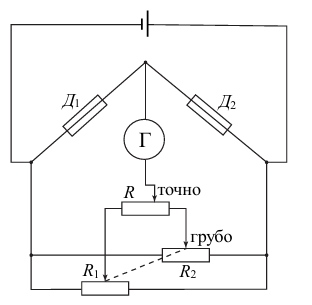
\includegraphics[width=0.5\textwidth]{img/most.png}
    
Измерительный мост
\end{center}
Мост балансируется, когда в сосудах находится только воздух при давлении близком к тому, при котором будут производиться измерения. Балансировка моста осуществляется с помощью переменных сопротивлений ($R, R_1, R_2$). Сопротивления $R_1, R_2$ спарены (их подвижные контакты находятся на общей оси) и изменяются одновременно при повороте ручки грубой регулировки. Точная регулировка выполняется потенциометром $R$. Балансировка закончена, когда показания гальванометра $\text{Г}$ влуктуируют около нулевого значения. При заполнении сосудов смесями различного состава возникает разбалансировка моста, и гальванометр показывает искомую разность напряжений на проволоках. Установка компьютеризирована, что позволяет снимать зависимость показаний гальванометра от времени с помощью программы.

\subsection{Таблица значений $\tau$ при различных давлениях}
\begin{tabular}{|c|c|c|c|c|c|}
    \hline
    $P, \text{торр}$ &  $\sigma_P, \text{торр}$ & $k\cdot 10^{-3}, \text{c}^{-1}$ & $\sigma_k\cdot 10^{-3}, \text{c}^{-1}$ & $\tau, \text{c}$ & $\sigma_\tau, \text{c}$ \\ \hline
    41  & 1.9 & -5.69  & 0.21  & 175.85  & 6.40 \\ \hline
    80  & 1.9 & -2.49  & 0.05  & 401.96  & 7.50 \\ \hline
    120 & 1.9 & -1.91  & 0.04  & 523.64  & 9.92 \\ \hline
    153 & 1.9 & -1.262 & 0.019 & 792.42  & 12.30 \\ \hline
    194 & 1.9 & -1.440 & 0.021 & 694.38  & 9.80 \\ \hline
    235 & 1.9 & -0.980 & 0.009 & 1020.30 & 8.87 \\ \hline
\end{tabular}

\subsection{Таблица значений $D$ при различных давлениях}
\begin{tabular}{|c|c|c|c|c|c|c|}
    \hline
    $P, \text{торр}$   & 41 & 80 & 120 & 153 & 194 & 235 \\ \hline
    $D, \frac{\text{см}^2}{c}$ & 11.67 & 5.10 & 3.92 & 2.59 & 2.95 & 2.01 \\ \hline
    $\sigma_D, \frac{\text{см}^2}{c}$ & 0.011 & 0.0022 & 0.0017 & 0.0009 & 0.0011 & 0.0006 \\ \hline
\end{tabular}
\subsection{Формулы для расчета погрешностей}
\subsubsection{Расчет погрешности углового коэффициента графика $ln(U)(t)$.}
\[\sigma_k = \frac{1}{\sqrt{n}}\sqrt{\frac{\langle ln(U)^2 \rangle - {\langle ln(U) \rangle}^2}{\langle t^2 \rangle - {\langle t \rangle}^2} - k^2}\] $n$ - количество экспериментальных точек.
\subsubsection{Расчет погрешности $\tau$.}
\[\epsilon_\tau = \epsilon_k \Rightarrow \frac{\sigma_\tau}{\tau} = \frac{\sigma_k}{k} \Rightarrow \sigma_\tau = \frac{\tau \cdot \sigma_k}{k}\]
\subsubsection{Расчет погрешности $D$.}
\[ \sigma_D = D\sqrt{{\epsilon_\tau}^2 + {\epsilon_{\frac{L}{S}}}^2 + {\epsilon_V}^2}\]
\subsubsection{Расчет погрешности углового коэффициента и свободного члена графика $D(\frac{1}{P})$.}
\[\sigma_k = \frac{1}{\sqrt{n}}\sqrt{\frac{\langle D^2 \rangle - {\langle D \rangle}^2}{\langle \frac{1}{P}^2 \rangle - {\langle \frac{1}{P} \rangle}^2} - k^2}\]
\[\sigma_b = \sigma_k \cdot \sqrt{\langle (\frac{1}{P})^2 \rangle - {\langle \frac{1}{P} \rangle}^2}\]
\subsubsection{Расчет погрешности $D_\text{атм}$.}
\[ \sigma_{D_\text{атм}} =\sqrt{\frac{\sigma_k^2}{P_\text{атм}^2} + \sigma_b^2}\]